\chapter{Model Architecture}

In this chapter, the architectures of several models are presented. Section \ref{modpoly} gives a comprehensive explanation to the structure of PolygonRNN, while section \ref{modfpn} looks into the FPN part of Mask R-CNN. Considering our problem, we combine PolygonRNN and FPN part of Mask R-CNN together and come up with a new model, which is called \modelnameshort\ (\modelnamelong, see section \ref{modmer}). In theory, the proposed model can find out the bounding boxes of buildings within an aerial image and give geometrical shape for each building.
 
\section{PolygonRNN}\label{modpoly}

PolygonRNN is the core model for finding geometrical shapes in this project. Figure \ref{fig:simppoly} shows the simplified structure of PolygonRNN. The CNN part (see subsection \ref{modcnn}) can capture image features through multilayer convolutions and max pooling, which is then fed into the RNN part (see subsection \ref{modrnn}), which can sequentially predict spatial location of the new vertex with the highest probability at each time step.

\begin{figure}[!h]
	\centering
	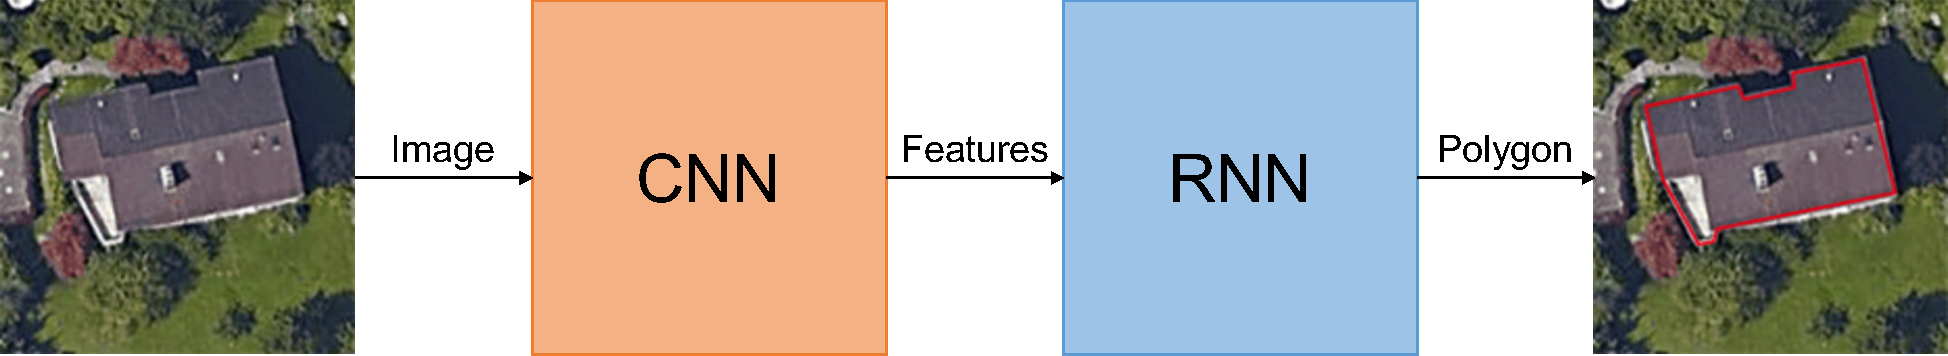
\includegraphics[width=\fig\textwidth]{3-00.pdf}
    \caption[The simplified model architecture of PolygonRNN]{The simplified model architecture of PolygonRNN.}
    \label{fig:simppoly}
\end{figure}

\subsection{CNN Part}\label{modcnn}

The CNN part of PolygonRNN uses VGG-16. Actually, VGG-16 is a form of VGGNet, which is very structured and focusing on deepening the  neural network without a large number of parameters. It generally believes that deeper networks have stronger expressive capabilities than shallow networks, and can accomplish more complex tasks. It also proven in practice that VGGNet has made great progress in performance compared to its previous network architecture (e.g. AlexNet).

The `16' in VGG-16 means that it is a VGGNet with 16 layers containing parameters (13 convolutional layers and 3 fully connected layers). It has around 138 million parameters in total. Figure \ref{fig:vgg16} shows its detailed network structure. From the figure we can see that VGG-16 continuously does convolution with $3\times3$ small kernels and makes $2\times2$ max pooling. As the network deepens, the width and height of the image are reduced by half after each max pooling, and the number of channels is also doubly increasing after some convolution.

\begin{figure}[!h]
	\centering
	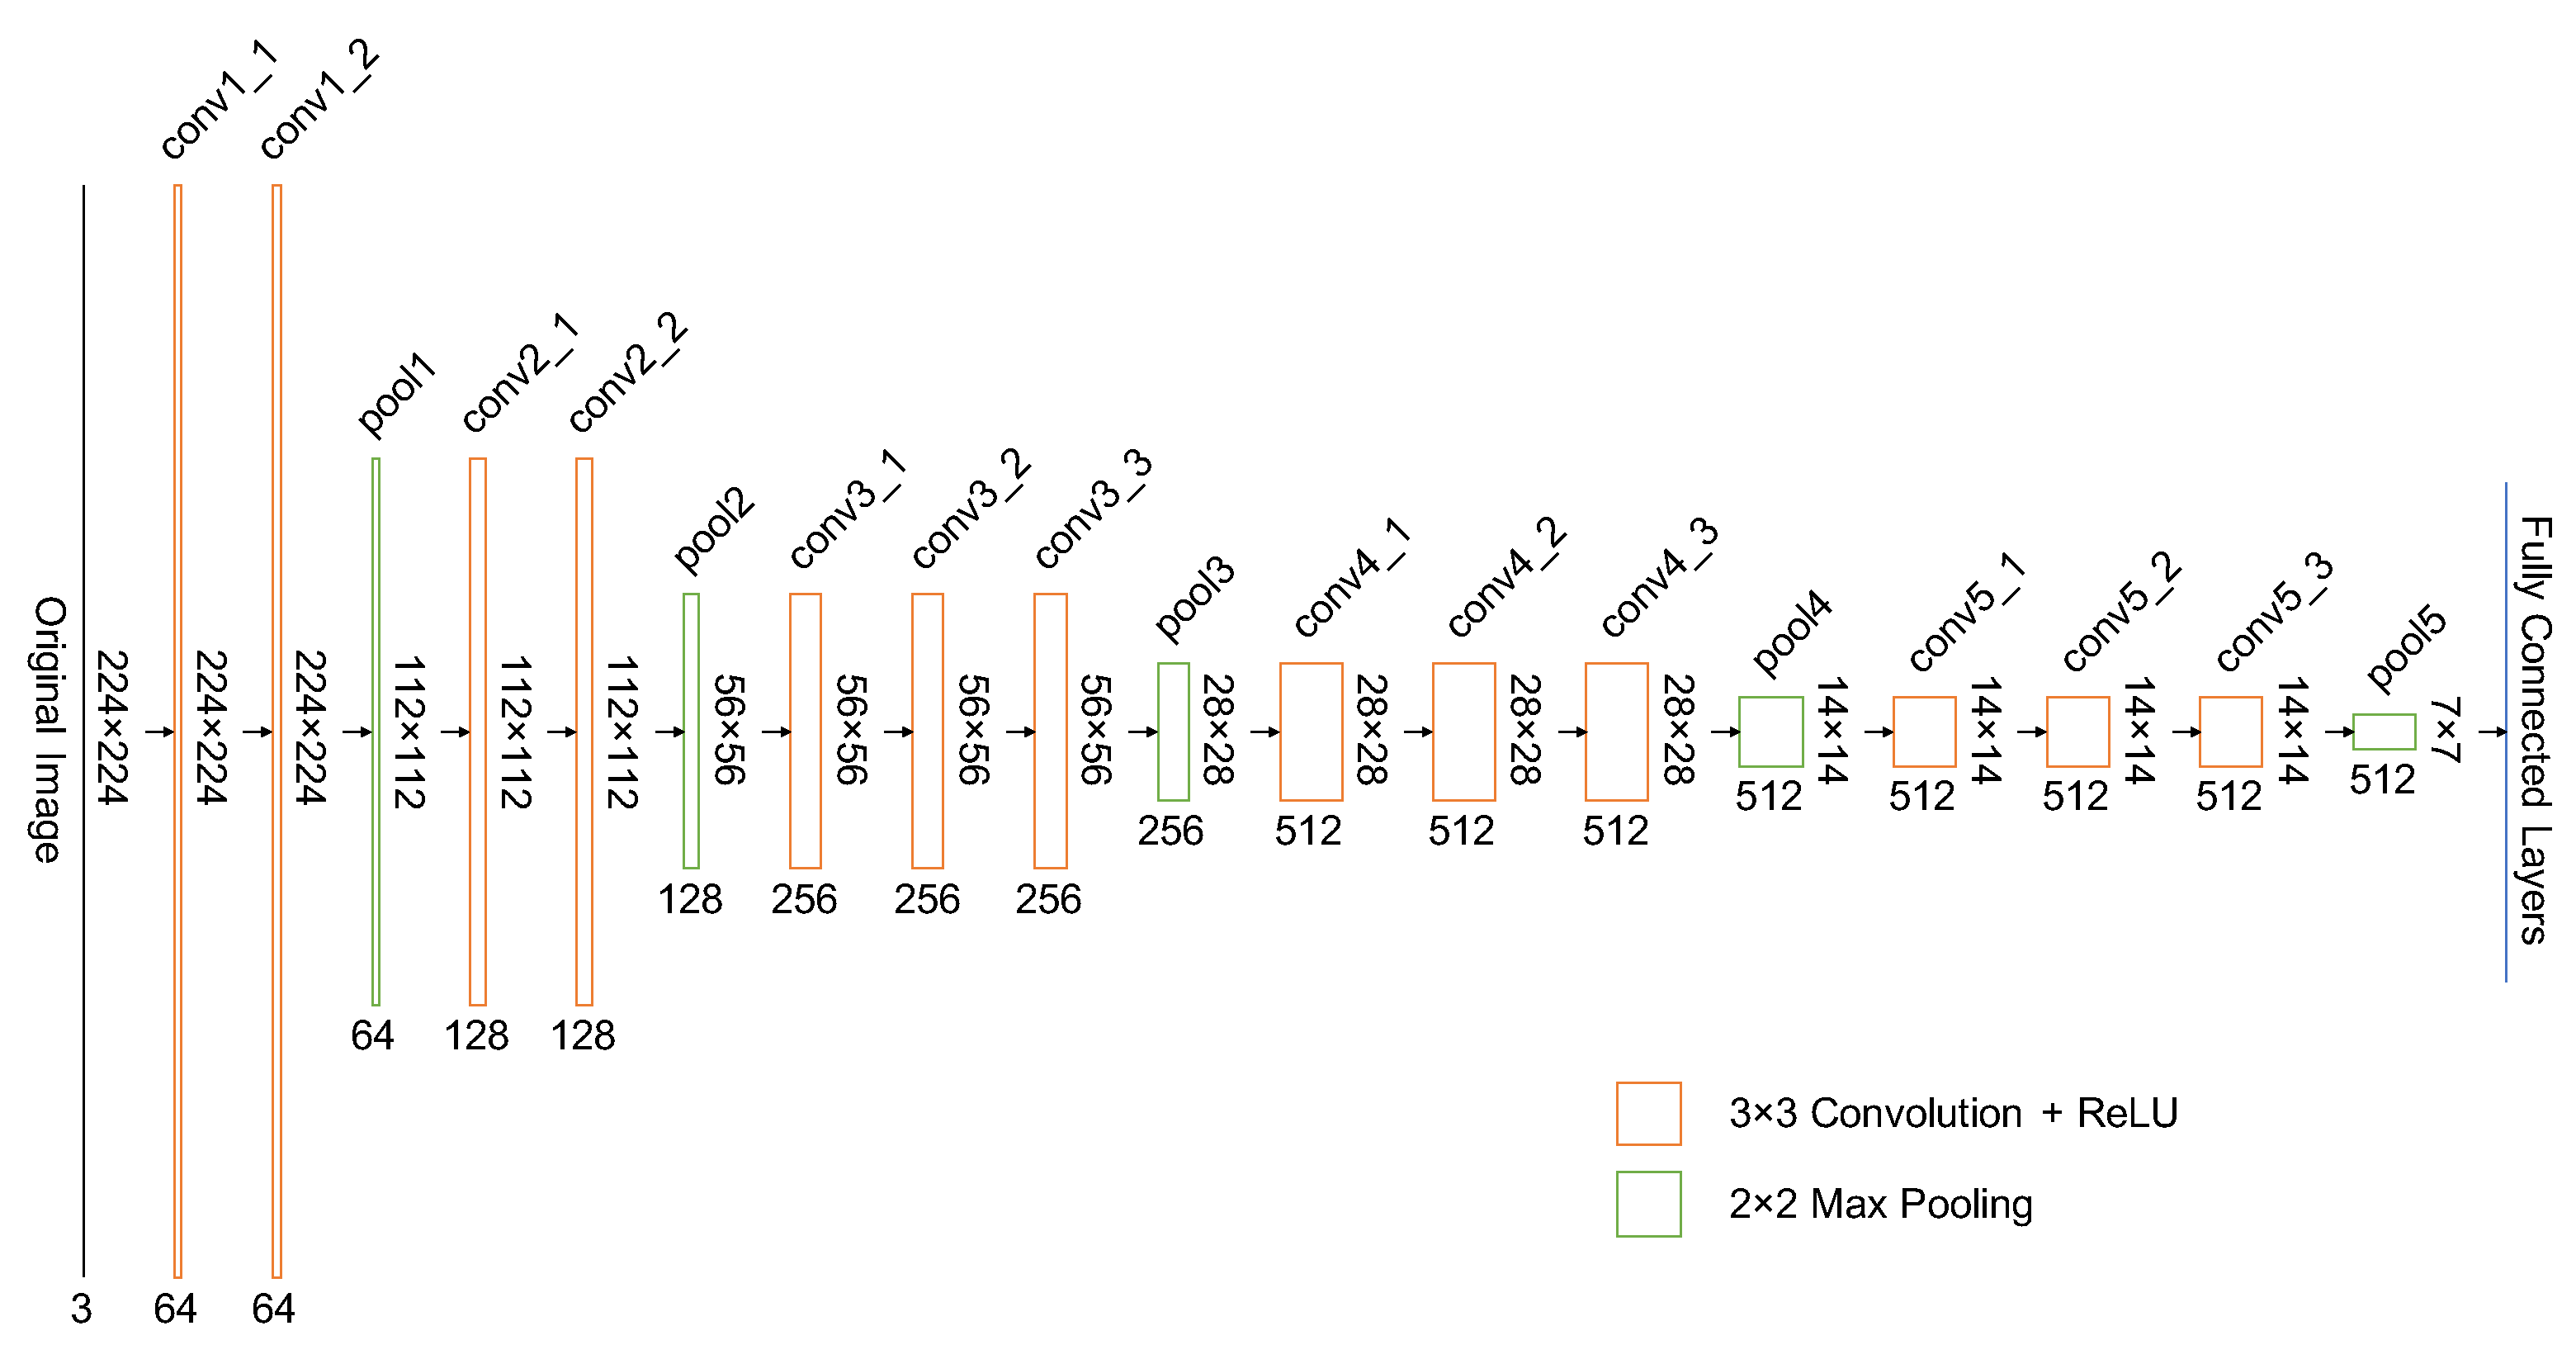
\includegraphics[width=\fig\textwidth]{3-01.pdf}
    \caption[VGG-16 architecture]{VGG-16 architecture. Only convolutional layers and maximum pooling layers are presented.}
    \label{fig:vgg16}
\end{figure}

VGG-16 was mostly used for image classification before, so after the convolutional layers and max pooling layers there are fully connected layers and softmax layer for the class labels. However, these two kinds of layers are not required for VGG-16 used in PolygonRNN, because the CNN here is working as a feature extractor and mask predictor. Layer \lstinline{pool5} is omitted as well because of the too low resolution.

\paragraph{Feature Extraction} The modified VGG-16 provides RNN with useful features, which are taken from different convolutional and max pooling layers. Specifically, the features are extracted from layer \lstinline{pool2}, \lstinline{pool3}, \lstinline{conv4_3} and \lstinline{conv5_3}. Note that since the resolution of final features is fixed, when taking features from layer \lstinline{pool2} and \lstinline{conv5_3}, it requires another max pooling and upsampling respectively. All of these can be seen in figure \ref{fig:mdfvgg16}.

\begin{figure}[!h]
	\centering
	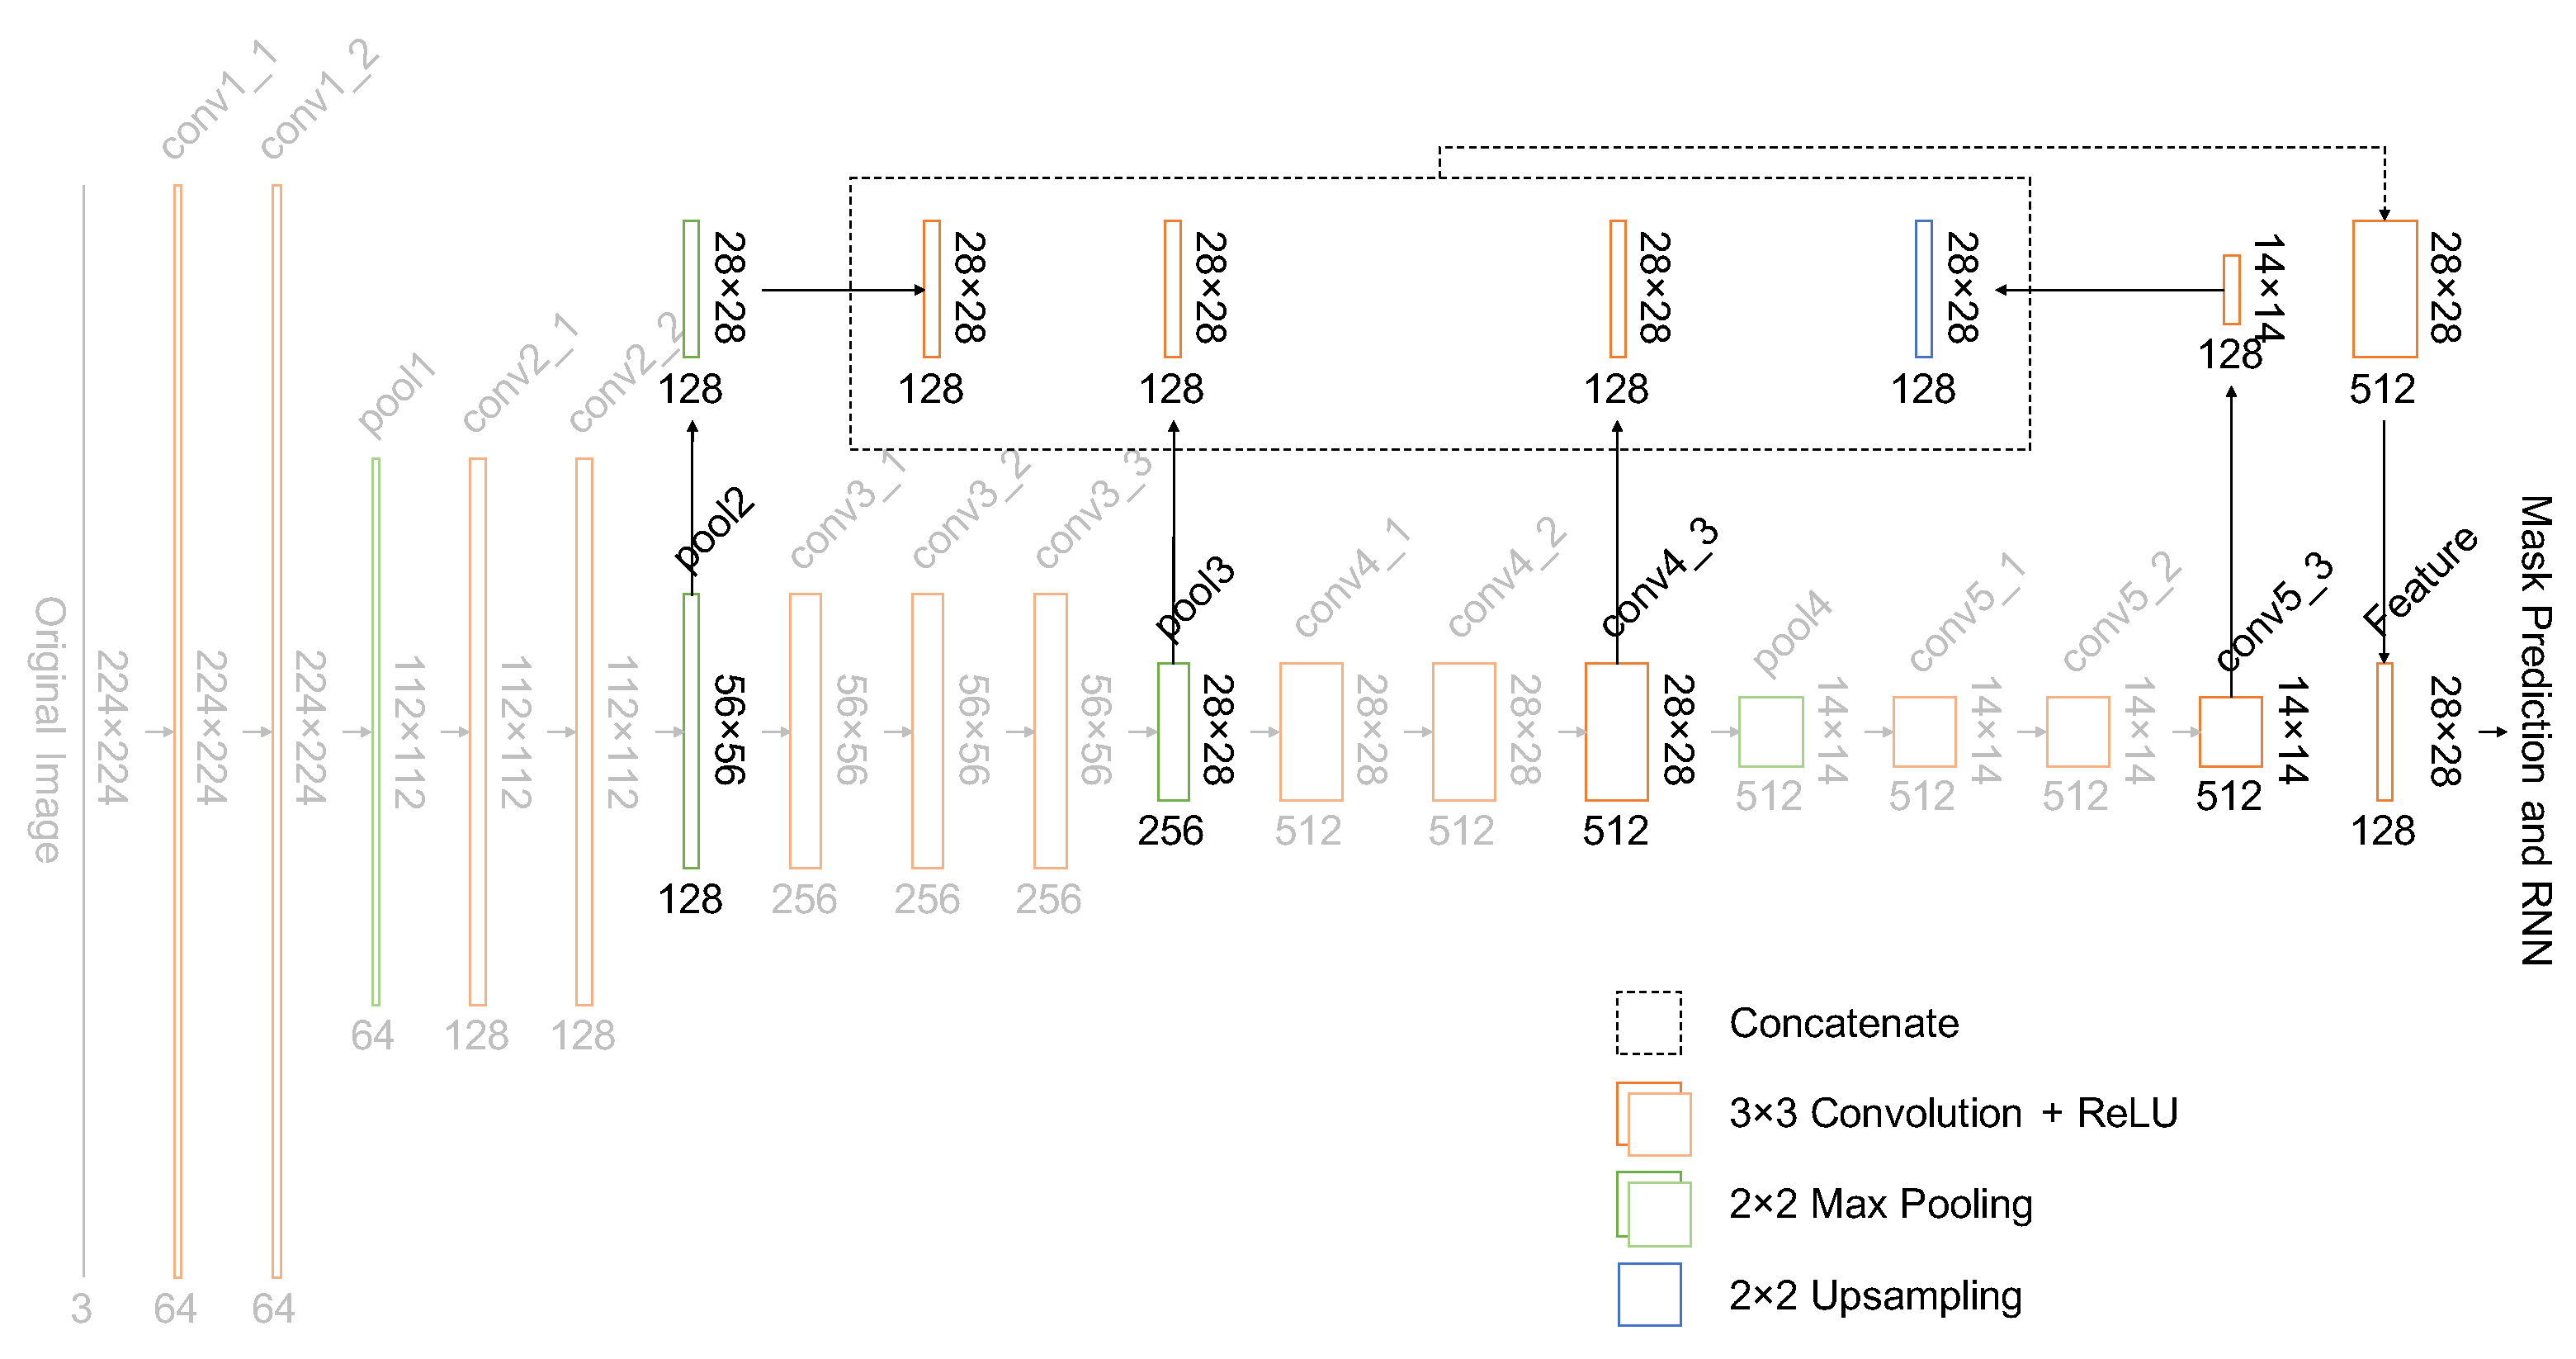
\includegraphics[width=\fig\textwidth]{3-02.pdf}
    \caption{Modified VGG-16 architecture in PolygonRNN.}
    \label{fig:mdfvgg16}
\end{figure}

\paragraph{Mask Prediction}
Another function of the CNN part is to predict masks of boundary and vertices in a low resolution (one eighth of the original). Figure \ref{fig:vgg16mask} shows the mask prediction phase. Different from the ReLU function used in the former convolutional layers, the activation function used here is the sigmoid function. Each entry of the boundary or the vertices mask indicates the probability that the pixel is located in the boundary or is a vertex respectively. The features and two masks are then sent into RNN together.
\begin{figure}[!h]
	\centering
	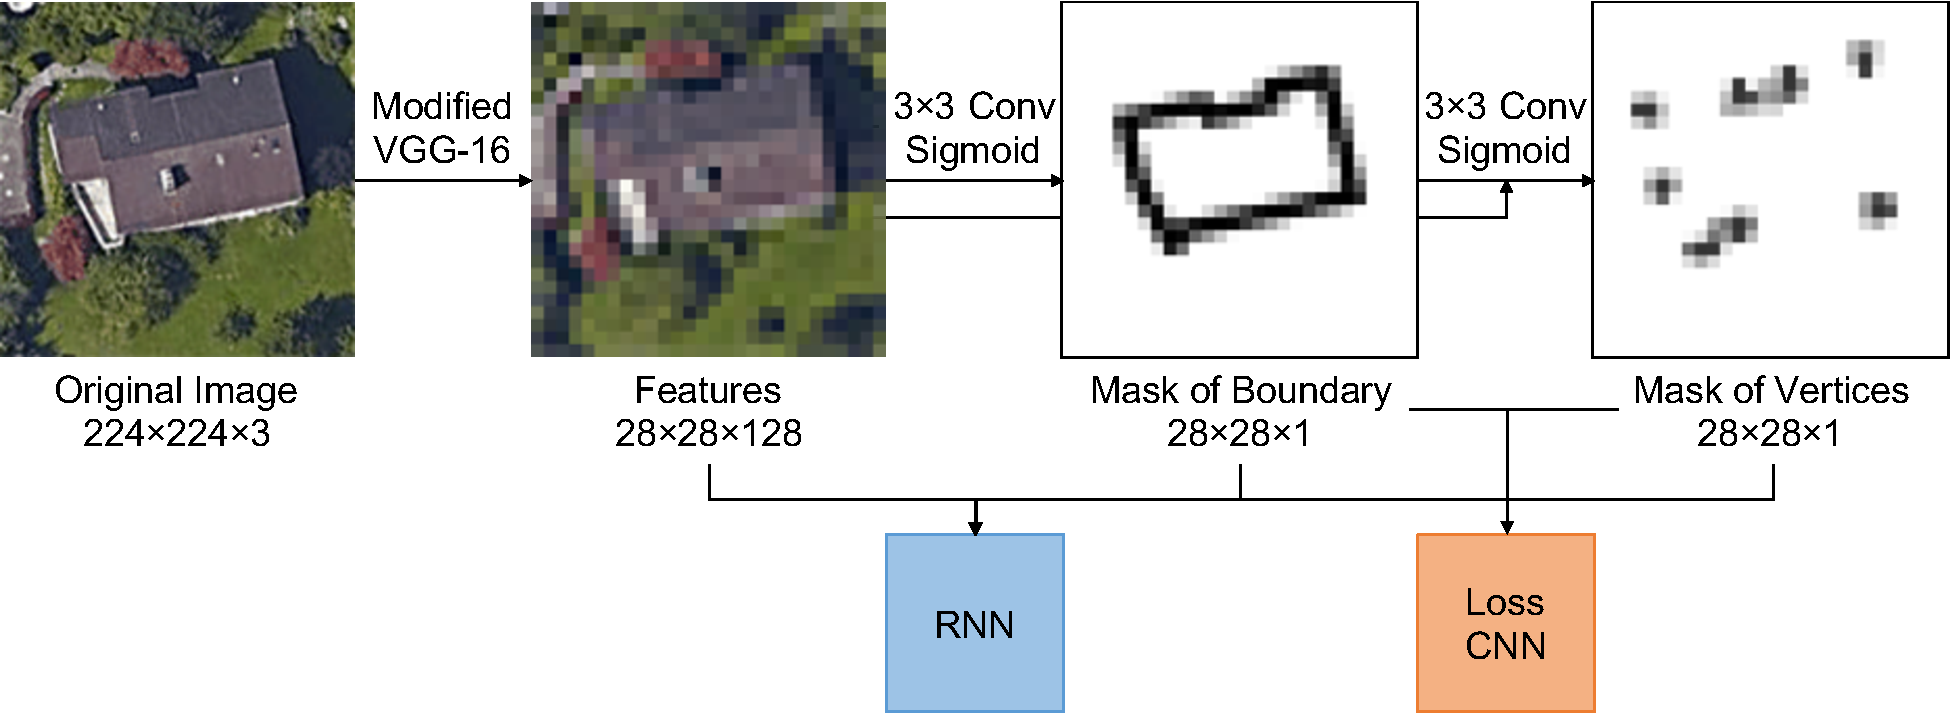
\includegraphics[width=\fig\textwidth]{3-03.pdf}
    \caption[Mask prediction of VGG-16]{Mask prediction of VGG-16. Note that the mask of vertices is obtained by the convolution on the concatenation of the features and the mask of boundary.}
    \label{fig:vgg16mask}
\end{figure}

\subsection{RNN Part}\label{modrnn}
The model used for predicting polygon vertices is RNN. We have already mentioned in subsection \ref{relatpoly} that RNN is very powerful when data is related to time series, and in our case, we regards the polygon as a series of vertices.

We know that given two vertices on a polygon in an order (either clockwise or anticlockwise), the third vertex after the two points can be uniquely determined. What RNN here can do is to predict the probability distribution of the next vertex's position in a low resolution when given the history information about the two vertices before, as well as the image features and the position of the starting vertex. This process can be formulated as follows.
\begin{equation}\label{eq:vnext}
	p(v_t|v_{t-1}, v_{t-2}) = F(v_{t-1}, v_{t-2}, v_0, p), \forall t \in \{2,3,4,...,T\},
\end{equation}
where $p$ denotes the extracted features by CNN (including the masks of boundary and vertices), $F(\cdot)$ denotes a function for computing the conditional probability, $T$ denotes the number of vertices of the polygon, $v_t$ denotes the vertex position at $t$-th prediction. Specifically, the vertex prediction problem can be formulated as a classification problem. The position of $v_t$ can be then quantized to the resolution of output grid, and we can thus use one-hot encoding for $v_t$'s representation.

\paragraph{End Signal} Note that the positions for $v_t$ are not only limited to the general output grid, the end signal for the closure detection of the polygon is also embedded in $v_t$, just like the `end of sequence' token \lstinline{<eos>} or \lstinline{</s>} in the RNN language model. Thus, the number possible assignments of $v_t$ equals to the resolution of the output grid plus one ($28\times28+1=785$ in our case). In order to correctly predict the end signal, the starting vertex $v_0$ is required for the conditional probability (equation \ref{eq:vnext}) calculation, as it tells the model when to finish the prediction phase. If the current prediction is the same as, or very close to the starting vertex $v_0$, $v_t$ will be forced to raise the end signal, indicating that the entire polygon is close, and the prediction phase is therefore complete. So generally, the end signal works when $t=T$.

\paragraph{Starting Vertex} In equation \ref{eq:vnext}, two special cases $p(v_0)$ and $p(v_1|v_0)$ are not included yet. These two cases are different from the general case, and should be considered in addition. In particular, we can directly regard the mask of vertices (for example, the rightmost image in figure \ref{fig:vgg16mask}) predicted by the CNN as $v_0$'s unnormalized probability distribution $\tilde{p}(v_0)$, and choose the position with the highest probability for $v_0$'s assignment. As $v_0$ is known, there are typically two options for $v_1$, one is the next vertex on its left direction and another on right direction. To tackle this problem, we can simply specify the order of the polygon vertices to be fixed, so that $v_1$ can be uniquely determined. In our project, the order of polygon is set to be anticlockwise.

\paragraph{ConvLSTM} The RNN uses ConvLSTM (Convolutional LSTM) cells as the polygon decoder to sequentially predict vertices. For simplicity, we can regard ConvLSTM as the function $F(\cdot)$ in equation \ref{eq:vnext}. In fact, the structure of a ConvLSTM cell is almost the same as that of an ordinary LSTM cell, except that it employs convolution in a 2D image with multiple channels instead of matrices or vectors multiplication. The introduction of ConvLSTM can significantly reduce the the number of parameters when it is compared with a fully connected RNN. The following equations define the computation process within a ConvLSTM cell, which is also visualized in figure \ref{fig:lstmcell}.
\begin{equation}
	\left[\begin{array}{c}
		f_t\\i_t\\g_t\\o_t
	\end{array}\right] = \left[\begin{array}{c}
		W_{hf}\\W_{hi}\\W_{hg}\\W_{ho}
	\end{array}\right] * h_{t-1} + \left[\begin{array}{c}
		W_{xf}\\W_{xi}\\W_{xg}\\W_{xo}
	\end{array}\right] * x_{t} + \left[\begin{array}{c}
		b_f\\b_i\\b_g\\b_o
	\end{array}\right] = W_h * h_{t-1} + W_x * x_t + b,
\end{equation}
\begin{equation}
	c_t = \sigma(f_t) \circ c_{t-1} + \sigma(i_t) \circ \tanh(g_t),
\end{equation}
\begin{equation}
	h_t = \sigma(o_t) \circ \tanh(c_t),
\end{equation}
where $x_t$, $h_t$, $c_t$ denote the input, the hidden state (or cell output), and the cell state of the cell at time step $t$ respectively, $i_t$, $o_t$, $f_t$ denote the states of input, output, and forget gate at time step $t$ respectively, $g_t$ denotes an intermediate variable, $\sigma(\cdot)$, $*$, $\circ$ denote the sigmoid function, convolution, and Hadamard (element-wise) product respectively, $W_x$ and $W_h$ denotes two convolution kernels for $x_t$ and $h_t$ respectively, $W_{xf}$, $W_{xi}$, $W_{xg}$, $W_{xo}$ denote the four components of $W_x$ and $W_{hf}$, $W_{hi}$, $W_{hg}$, $W_{ho}$ denote the four components of $W_h$.

\begin{figure}[!h]
	\centering
	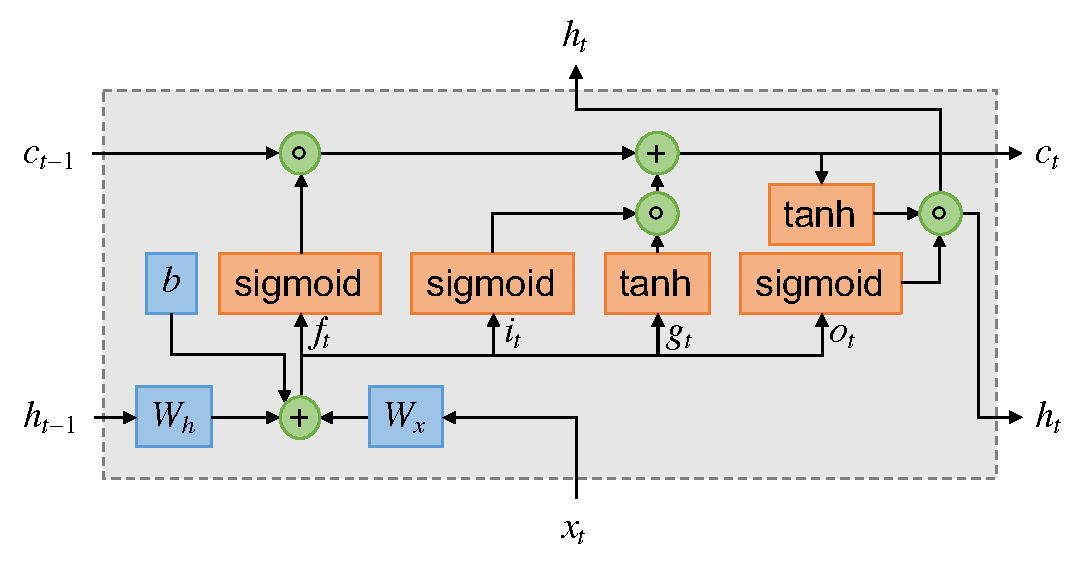
\includegraphics[width=\fig\textwidth]{3-04.pdf}
    \caption{Visulization for LSTM cell.}
    \label{fig:lstmcell}
\end{figure}

\paragraph{Multilayer RNN}
PolygonRNN uses multilayer RNN with ConvLSTM cells. The connection between two neighboring layers can be described as follows, which means that the cell input of this layer comes from the cell output of the previous layer.
\begin{equation}\label{eq:cellconnect}
	x_t^{(k)} = h_t^{(k-1)}, \forall k \in \{2,3,...,n\},
\end{equation}
where $n$ is the number of RNN layers or ConvLSTM cells, $k$ in the superscript denotes the $k$-th layer. Recall that the initial cell input (i.e. the cell input of the first layer) at time step $t$ consists of the spatial information $p$ from CNN, the two previous vertices $v_{t-1}$ and $v_{t-2}$, and starting vertex $v_0$, here it is formulated as follows.
\begin{equation}\label{eq:concat}
	x_t = x_t^{(1)} = v_{t-1} \oplus v_{t-2} \oplus v_0 \oplus p,
\end{equation}
where $\oplus$ denotes the concatenation operation in the dimension of image channel. Thus, the equation \ref{eq:vnext} can be written as follows.
\begin{equation}\label{eq:probcomp}
	y_t = p(v_t|v_{t-1}, v_{t-2}) = \softmax(W_y\vect(h_t^{(n)})),
\end{equation}
where $W_y$ denotes the weights of the final fully connected layer. Figure \ref{fig:rnnconvlstm} shows the entire structure of the RNN part and highlights the process at time step $t$, using the same notation as the equations \ref{eq:cellconnect}, \ref{eq:concat} and \ref{eq:probcomp}.

\begin{figure}[!h]
	\centering
	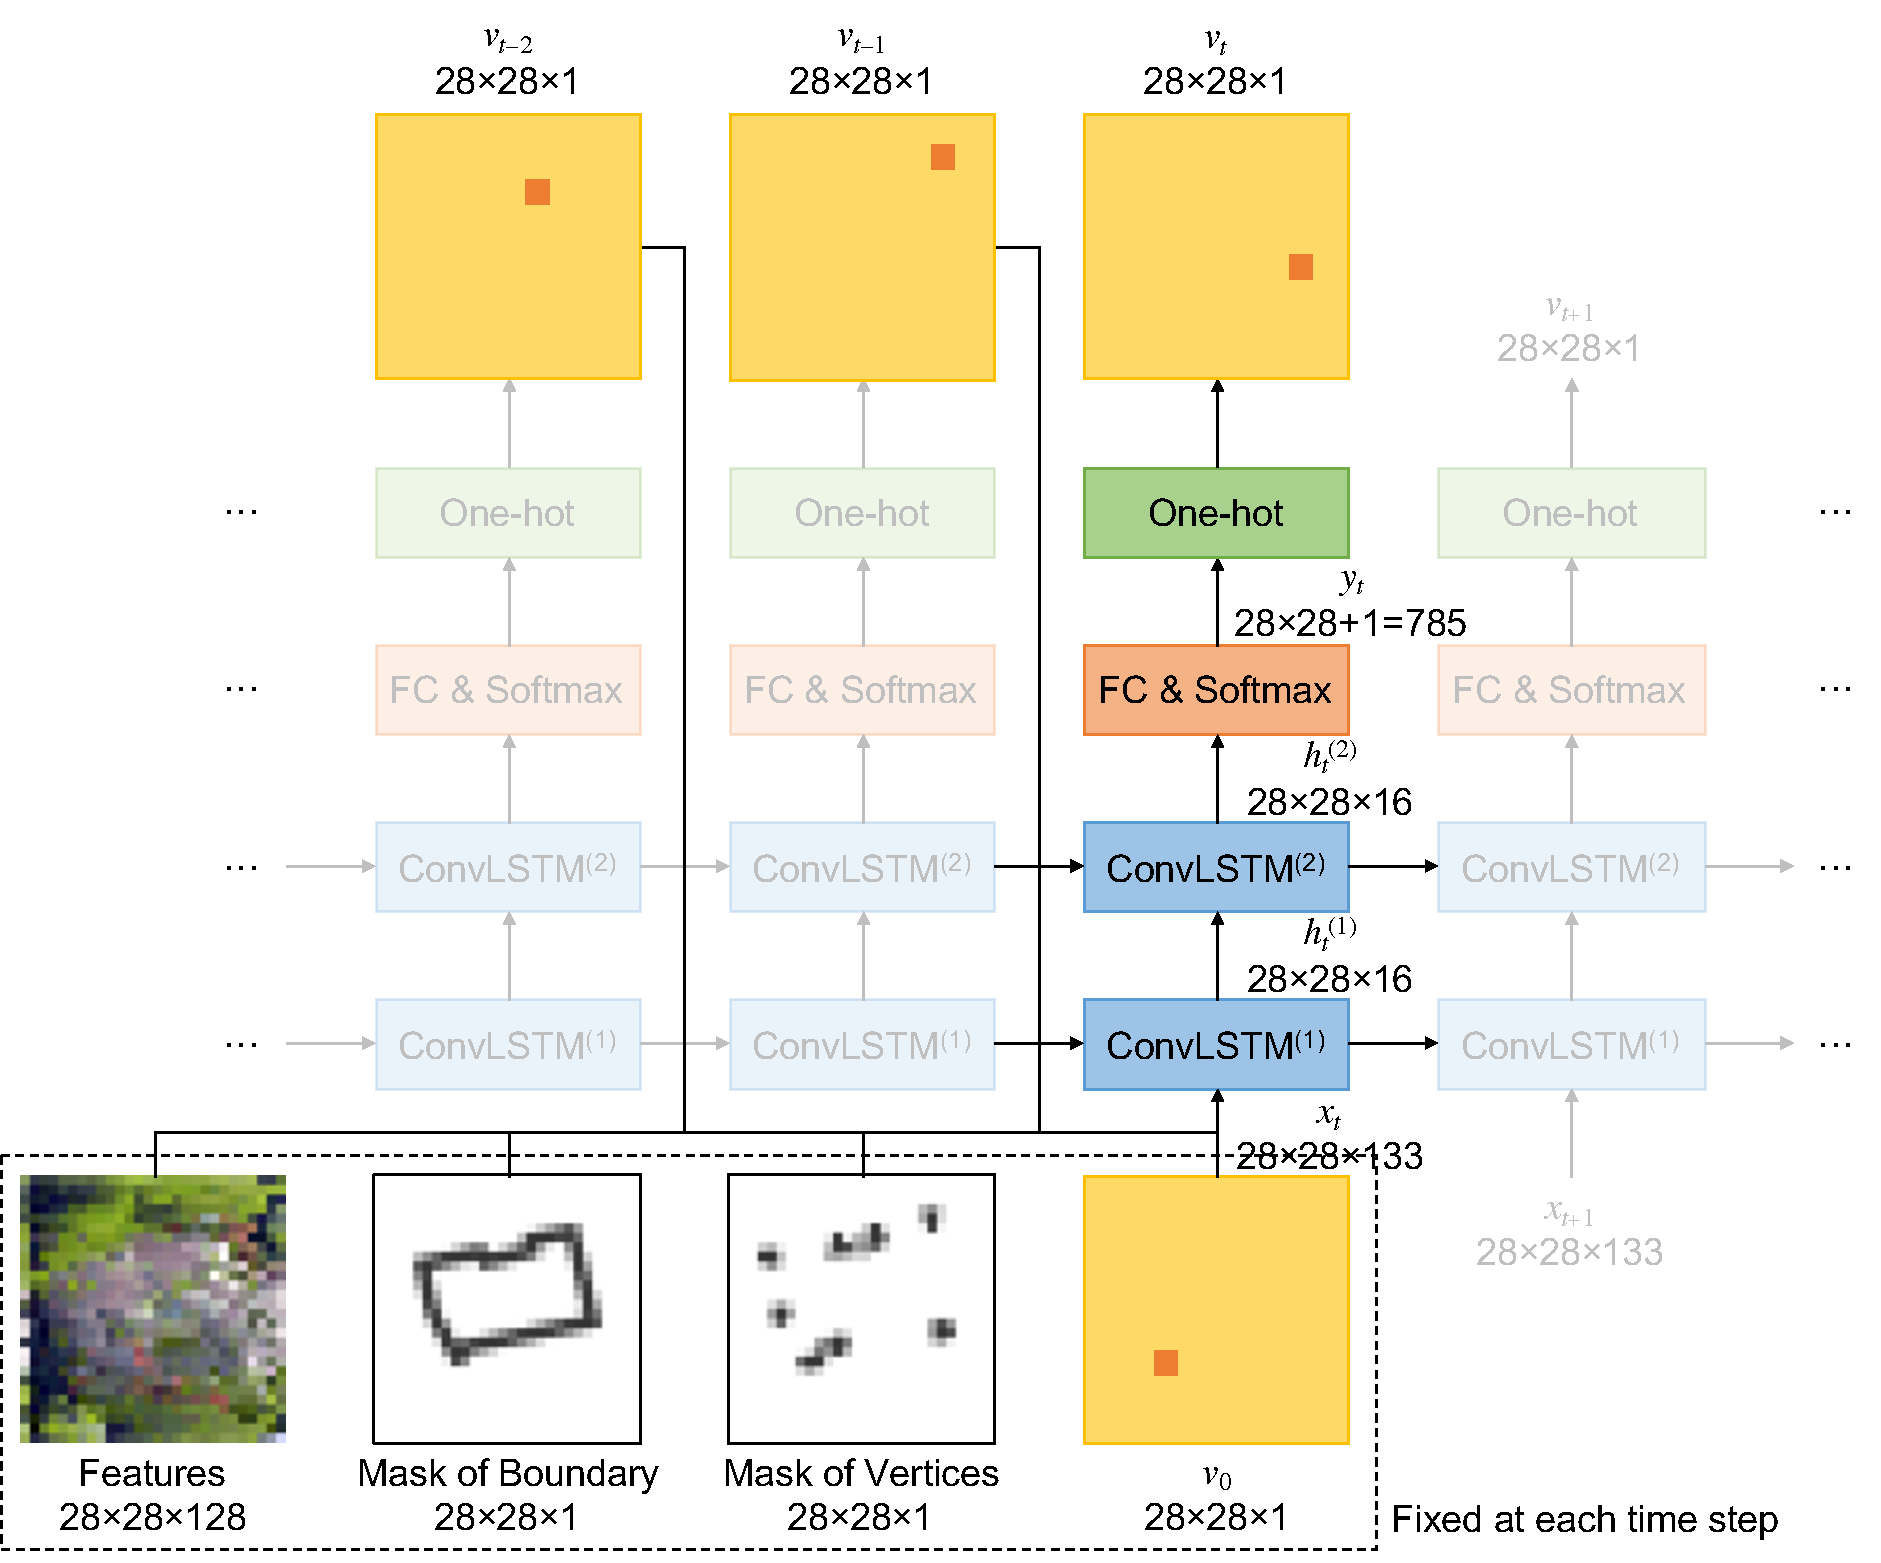
\includegraphics[width=\fig\textwidth]{3-05.pdf}
    \caption[Visualization for the time step of the RNN decoder]{Visualization for the time step of the RNN decoder. In this figure, the outputs of the end signal are omitted, and the configuration of the ConvLSTM cell is the same as what is used in the original PolygonRNN paper. Specifically, the paper sets the number of RNN layers to 2 and uses ConvLSTM cells with 3$\times$3 kernel size and 16 channels.}
    \label{fig:rnnconvlstm}
\end{figure}

\subsection{Loss Function}
The loss of PolygonRNN consists of two parts, loss of CNN and loss of RNN. The loss function of CNN part uses log loss, since the mask prediction is equivalent to binary classification for each pixel. We also notice that the non-boundary pixels or the non-vertex pixels occupy the majority, the loss function should be further weighted. As for the loss of RNN, the loss function used is cross-entropy loss, because the polygon prediction is equivalent to multiclass classification at every time step.

\section{Feature Pyramid Network}\label{modfpn}

FPN uses a top-down architecture with lateral connections to build an in-network feature pyramid from a single-scale input. Faster R-CNN with an FPN back- bone extracts RoI features from different levels of the fea- ture pyramid according to their scale, but otherwise the rest of the approach is similar to vanilla ResNet. Using a ResNet-FPN backbone for feature extraction with Mask R- CNN gives excellent gains in both accuracy and speed. For further details on FPN, we refer readers to [27].

For the network head we closely follow architectures presented in previous work to which we add a fully con- volutional mask prediction branch. Specifically, we ex- tend the Faster R-CNN box heads from the ResNet [19] and FPN [27] papers. Details are shown in Figure 3. The head on the ResNet-C4 backbone includes the 5-th stage of ResNet (namely, the 9-layer ‘res5’ [19]), which is compute- intensive. For FPN, the backbone already includes res5 and thus allows for a more efficient head that uses fewer filters.
We note that our mask branches have a straightforward structure. More complex designs have the potential to im- prove performance but are not the focus of this work.


\subsection{Anchor}

\subsection{Single Bounding Box Regression}

\subsection{Feature Pyramid}

Dummy text.

\section{\modelnameshort}\label{modmer}

Dummy text.

\subsection{Two-step Model}

Dummy text.

\subsection{Hybrid Model}

Dummy text.

\subsection{Hybrid Model with RoI Align}




